\chapter{Implementacja symulacji}
\label{cha:implementacja}
W tym rozdziale chciałbym przedstawić technologie i narzędzia użyte do wykonania symulacji oraz sposoby ich uruchomienia.
%---------------------------------------------------------------------------

\section{Środowisko QT}
\label{sec:qt}
{\color{red} CHECK}
Zdecydowałem się wykorzystać QT Creator IDE z kilku powodów, które zamierzam zaraz rozwinąć. Najważniejszą cechą środowiska jest udostępnienie go na kilku rodzajach licencji. Osobiście użyłem licencji LGPL, która pozwoliła mi bez ponoszenia kosztów korzystać ze środowiska. Kolejnym ważnym elementem jest multiplatformowość pozwalająca w łatwy sposób przenosić kod program między systemami operacyjnymi, o ile nie zostały użyte biblioteki dostępne tylko na jeden z systemów. Kolejną z zalet jest łatwy i intuicyjny interfejs tworzenia graficznego interfejsu użytkownika, osoba mająca wcześniej styczność z chociażby biblioteką Swing Java'y nie powinna mieć problemu z zaadaptowaniem się do  formularza QT Creatora. Wykorzystywany jest model sygnałów i slotów, polegający na emitowaniu sygnału przez zdarzenie, który następnie trafia do podłączonego slotu. Jest to w stanie znacznie ułatwić komunikację między elementami. Używanie nowoczesnego języka C++ (ja używałem wersji 14) nie sprawia problemów, lecz powinniśmy być świadomi że przykładowe uruchomienie wątków w aplikacji powinno być zrobione przy użyciu klas i funkcji z biblioteki QT.

%-------------------------------------------------------------------------------------------------------------------------------------------------------------

\section{QGLWidget}
\label{sec:glwidget}

%-------------------------------------------------------------------------------------------------------------------------------------------------------------

\section{Schemat programu}
\label{sec::schemat}
Rysunek \ref{fig:schemat} przedstawia poglądowy schemat działania programu. Dzieląc rysunek na lewą i prawą część możemy wyodrębnić dwa wątki. Po lewej wątek odpowiadający za wykonanie symulacji, po prawej wątek odpowiadający za rysowanie. Określeniem "Zasób" opisuję współdzielone dane ( opisane w podrozdziale \ref{sec::kod}) między wątkami, którymi jest historia symulacji. 

Podczas startu programu zostaje narysowany sześcian, po czym program przechodzi w stan nasłuchiwania na sygnały. Przykładowymi sygnałami mogą być zmiana rozmiaru okna aplikacji, bądź obrót figury. Po wykryciu takowego, następują próby zablokowania dostępu do zasobu dopóki nie zostanie to wykonane (zasób może być zablokowany przez inny wątek). Następnie na podstawie historii symulacji i/lub sygnału dokonywane jest nowe rysowanie. Po czym zasób zostaje zwolniony, a główny wątek (odpowiedzialny za rysowanie) wraca do stanu nasłuchiwania. 
\begin{figure}
    \centering
    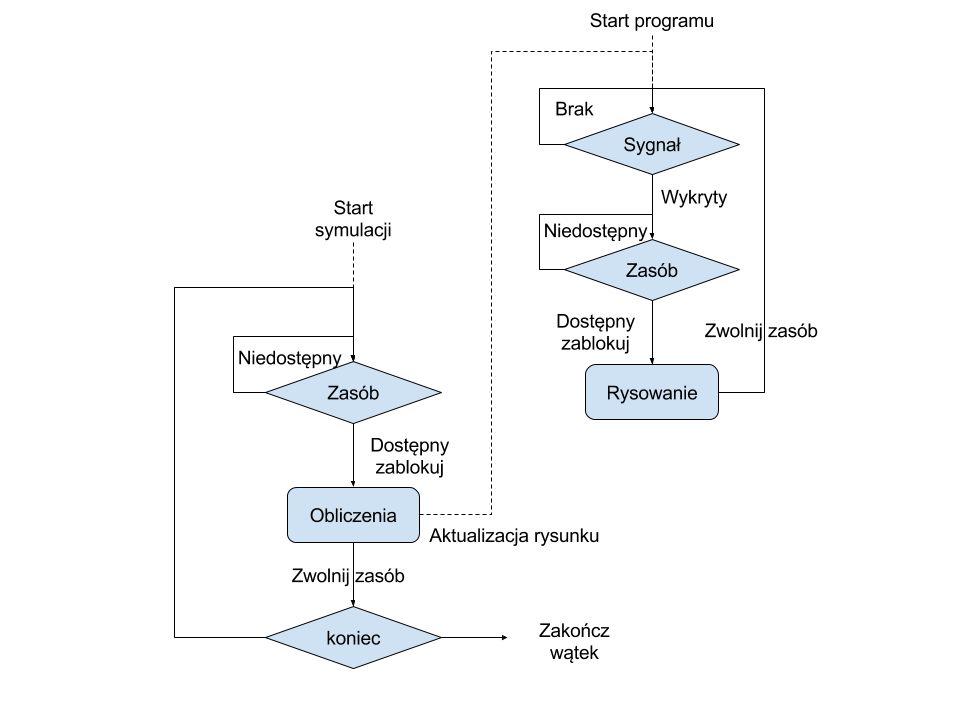
\includegraphics[width=0.9\textwidth]{pict/schemat.png}   
    \caption{Schemat programu}
	\label{fig:schemat} 
\end{figure}
Podczas startu symulacji (spowodowanej naciśnięciem przycisku \texttt{RUN}) identycznie poprzednio musi być uzyskany dostęp do zasobów. Dopiero po tym możliwe jest przeprowadzenie symulacji po jednej partii dla każdej instancji gry. Następnie zostaje to zapisane do zasobów, które zostają zwolnione. Równocześnie do wątku głównego wysyłany jest sygnał mówiący o aktualizacji historii symulacji. Jeśli była to ostatnia planowana partia wątek kończy swoje działanie.
%-------------------------------------------------------------------------------------------------------------------------------------------------------------

\section{Sygnały, sloty i mutex}
\label{sec::sig_slot}

%-------------------------------------------------------------------------------------------------------------------------------------------------------------

\section{Kod}
\label{sec::kod}
W tym podrozdziale będą opisane kluczowe fragmenty kodu, niezbędne do zrozumienia implementacji programu. Współdzielonymi zasobami są:
\begin{lstlisting}
template<typename T> using tup3= tuple<T,T,T>;
vector<vector<tup3<double>>> beginsp; //wektor punktów początkowych odcinków
vector<vector<tup3<double>>> endsp; //wektor punktów końcowych odcinków
vector<tup3<int>>colorsp;
mutex points;
\end{lstlisting}

\paragraph{Interfejs klasy \texttt{Game}}
Cała symulacja przeprowadzana jest w klasie \texttt{Game}, dlatego chciałbym ją teraz omówić. Reprezentuje ona jedną instancję gry 3-osobowej. Parametrem konstruktora jest indeks tablicy \texttt{decision\_funs}, której element zostaje przypisany do \texttt{decision}. \texttt{function} jest wrapperem biblioteki standardowej dla dowolnej funkcji, wyrażenia lambda, wyrażenia bind, funkcjonału lub wskaźników do funkcji. W poniższym kodzie \texttt{function} jest parametryzowany bezargumentowym, bezwynikowym zachowaniem. Funkcja \texttt{next} przeprowadza rozgrywkę jednej partii. Jej implementacja zostanie przedstawiona później. Zmienna \texttt{current} odpowiada $liczba_{partii}$, natomiast \texttt{nr[i]} odpowiada $nast_i$ (opisano w podrozdziale \ref{sec:model}). Funkcja \texttt{checker} jest odpowiednikiem funkcji $ogr$ (opisano w podrozdziale \ref{sec:ograniczenie}). Tablica \texttt{decision\_funs} zawiera funkcje lambda mające dostęp do prywatnych zmiennych klasy \texttt{Game}. W tablicach \texttt{result} znajdują się obliczone $\Delta p_i$, które następnie poddawane są funkcji ograniczającej. 

\begin{lstlisting}
class Game{
public:
    Game(int f);
    tup3<double> next();
    int getCurrent(); //zwraca numer bieżącej partii
    tup3<double> prelast(); //zwraca pre
private:
    array<double,3> p; //prawdopodobieństwa
    tup3<double> pre; //ostatnia krotka prawdopodobieństw na podstawie, których było dokonane losowanie sojuszników
    int current; //numer bieżącej partii
    array<int,3> nr;
    double checker(double r);
    function<void()> decision; //dokonuje modyfikacji prawdopodobieństw
    array<function<void()>,2>decision_funs={{
      [this](){//standardowe
        array<double,3> result= {
            0.1*( 1 - static_cast<double>(nr[1])/current - static_cast<double>(nr[2])/current),
            0.1*( 1 - static_cast<double>(nr[2])/current - static_cast<double>(nr[0])/current ),
            0.1*( 1 - static_cast<double>(nr[0])/current - static_cast<double>(nr[1])/current )
        };
        for(int i=0; i<3; i++)
            p[i]= checker(p[i]+result[i]);
      },
      [this](){//replikatorów
        array<double,3> result= {
            0.1*(p[0]*(1-p[0])*(1-static_cast<double>(nr[1])/current-static_cast<double>(nr[2])/current)),
            0.1*(p[1]*(1-p[1])*(1-static_cast<double>(nr[0])/current-static_cast<double>(nr[2])/current)),
            0.1*(p[2]*(1-p[2])*(1-static_cast<double>(nr[0])/current-static_cast<double>(nr[1])/current))
        };
        for(int i=0; i<3; i++)
            p[i]= checker(p[i]+result[i]);
      }
    }};
};
\end{lstlisting}

\paragraph{Implementacja \texttt{Game::next}}
Tablica \texttt{choices} zawiera losowe wartości dla każdego z zawodników, na podstawie których dokonywane jest losowanie sojusznika.
\begin{lstlisting}
tup3<double> Game::next(){
    pre= make_tuple(p[0],p[1],p[2]);
    current++;
    array<double,3> choices= {static_cast<double>(rand())/RAND_MAX, static_cast<double>(rand())/RAND_MAX, static_cast<double>(rand())/RAND_MAX};
    for(int i=0; i<3; i++)
        if(choices[i]<p[i])
            nr[i]++;
    decision();
    return make_tuple(p[0],p[1],p[2]);
}
\end{lstlisting}

\paragraph{Implementacja wątku symulującego} \texttt{QtConcurrent::run} jest funkcją uruchamiającą w osobnym wątku funkcję podaną jako parametr. Zwraca ona obiekt \texttt{QFuture}, który nie może przerwać lub wstrzymać wątku. Poprzez \texttt{beginsp.resize(p)} tworzony jest wektor posiadający p pustych elementów(wektorów krotek), ponieważ już w pierwszej partii będziemy potrzebować osobnego wektora dla każdej instancji gry. Natomiast \texttt{beginsp[i].reserve(g)} rezerwuje pamięć dla g partii, gdyby ta funkcja nie została użyta prawdopodobnie wystąpiłaby realokacja pamięci, w celu zapewnienia jej ciągłości. Przekładałoby się to na spowolnienie działania programu. Napisałem prawdopodobnie, ponieważ standard języka nie precyzuje ilości pamięci domyślnie rezerwowanej przez wektor, co jest zostawione po stronie implementacji. Przed wykonaniem każdej partii wątek czeka na dostęp do zasobu. Funkcja \texttt{try\_lock()} zwróci \texttt{true} w przypadku udanego przydzielenia zasobu, w przeciwnym razie zwróci \texttt{false}. 
\begin{lstlisting}
QtConcurrent::run(
            [&]()->void{
                ui->pushButton_Run->setEnabled(false);
                const int g= nr_rounds;
                const int p= nr_players;
                const int f= fun;
                vector<unique_ptr<Game>> tab;
                std::default_random_engine generator;
                std::uniform_int_distribution<int> distribution(0,255);
                auto r= bind(distribution, generator);
                clear_vectors();
                chrono::milliseconds d(delay);
                beginsp.resize(p);
                endsp.resize(p);
                for(int i=0; i<p;i++){
                    tab.push_back(make_unique<Game>(f));
                    colorsp.push_back(make_tuple( r(), r(), r() ));
                    beginsp[i].reserve(g);
                    endsp[i].reserve(g);
                }
                for(int j=0; j<g;j++){
                    if(quit) return;
                    while(!points.try_lock());
                    for(int i=0; i<p;i++){
                        beginsp[i].push_back(tab[i]->next());
                        endsp[i].push_back(tab[i]->prelast());
                    }
                    points.unlock();
                    emit copy();
                    this_thread::sleep_for(d);
                }
                ui->pushButton_Run->setEnabled(true);
            });
\end{lstlisting}

%-------------------------------------------------------------------------------------------------------------------------------------------------------------

\section{Rysowanie 3D}
\label{sec::3d}

%-------------------------------------------------------------------------------------------------------------------------------------------------------------

\section{Makefile}
\label{sec::makefile}
Symulując grę w okręgu postanowiłem rysować wykresy funkcji prawdopodobieństwa od numeru partii. Do tego celu uznałem, że najbardziej odpowiedni będzie plik \texttt{Makefile}, który wykona kompilację, uruchomienie oraz narysowanie wykresu przy pomocy programu gnuplot. Aby uruchomić program należy podać argument: G - ilość partii do rozegrania oraz P - ilość graczy. Poniżej przykładowe polecenie do wykonania symulacji dla 100 partii rozegranych przez 20 zawodników.
\begin{verbatim}
make G=100 P=20
\end{verbatim}
Wymagany kompilator g++ ver.5+ oraz gnuplot. 
